\documentclass{standalone}
\usepackage{tikz}
\usetikzlibrary{shapes.geometric, arrows}

\begin{document}
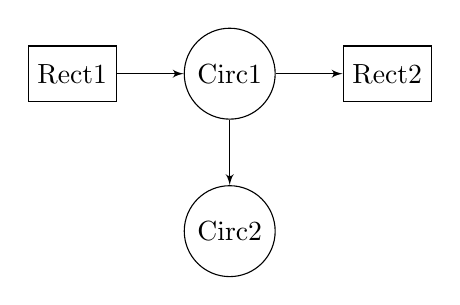
\begin{tikzpicture}[node distance=2cm, auto]
  % Define style for boxes
  \tikzstyle{rect} = [rectangle, draw, text centered, minimum height=2em]
  \tikzstyle{circ} = [circle, draw, text centered, minimum size=2em]
  \tikzstyle{line} = [draw, -latex']

  % Place nodes
  \node [rect] (rect1) {Rect1};
  \node [circ, right of=rect1] (circ1) {Circ1};
  \node [rect, right of=circ1] (rect2) {Rect2};
  \node [circ, below of=circ1] (circ2) {Circ2};
  % other nodes here

  % Draw edges
  \path [line] (rect1) -- (circ1);
  \path [line] (circ1) -- (rect2);
  \path [line] (circ1) -- (circ2);
  % other paths here
\end{tikzpicture}
\end{document}
